
As a cross-check to the BDT analysis, an analysis with sequential
selection cuts is performed. Since the signal region of such a cut-based
analysis is more easily understood, it is an important test of the
predictions of the BDT analysis. Morever, comparing the SRs of the
cut-based analysis to those of the BDT results in a better
understanding of BDT analysis. 

\subsection{Selection}

The essential difference between the BDT analysis and the cut-based
approach is that instead of training a BDT classifier with eight
discrimating independent variables, binary cuts are placed on these
variables. In the cut-based analysis, all BDT inputs are used, with
the exception of \SumMlj and \lepEtaCent, since cutting on these two has been
shown to yield little sensitivity improvement. Cut values are
determined in a simultaneous optimization procedure, and the resulting
cuts are shown in
table~\ref{chap:analysis:tab:cutbased_selection}. The same common
pre-selection cuts are
applied for both the BDT and cut-based analysis. Apart from the
\etmiss cuts, which are tighter for cut-based, the same VBF-specific
pre-selection cuts are applied as well. Upon applying the cuts
sequentially, a binned likelihood fit is performed on the \mT
distribution, with optimized bin boundaries of [0,80,130,$\infty$]. In
addition to an $\mjj > 600 \gev$ cut, the \mT fit is split into a $600
< \mjj < 1000 \gev$ bin and a $\mjj > 1000 \gev$ bin to exploit the
larger $S/B$ in the $\mjj > 1000 \gev$ region. 

\begin{table}[h]
\centering
\renewcommand{\arraystretch}{1.1}
\begin{tabular}{c|c}
\hline
\multirow{4}{0.15\textwidth}{Common pre-selection} &  $p_{\textrm{T1}(T2)} >$~22(10)~$\gev$ \\
 &  $\mll > 10(12) \gev$ for \emme (\eemm) \\
 &  opposite charge leptons    \\
 &  $|\mll - m_Z|>15 \gev$    \\
\hline
 \multirow{6}{0.15\textwidth}{Background rejection} &  $\Njet \geq 2$    \\
 &  $\calomet > 55 \gev$ (\eemm)    \\
 &  $\trkmet > 50 \gev$ (\eemm)   \\
 &  $\Nbjet = 0$    \\
 &  $\pTtot < 15 \gev$    \\
 &  \Ztau~veto    \\
\hline
 \multirow{4}{0.15\textwidth}{VBF topology} &  CJV    \\
 &  OLV    \\
 &  $\dyjj > 3.6$   \\
 &  $\mjj > 600 \gev$, split at $1 \tev$ \\
\hline
 \multirow{4}{0.15\textwidth}{Higgs decay topology}    &  $\mll < 50 \gev$ \\
 &  $\dphill < 1.8$ ($p_{\textrm{T2}} > 15 \gev$) \\
 &  $\dphill < 2.8$ ($10 < p_{\textrm{T2}} < 15 \gev$) \\
 &  Fit \mT distribution \\
\hline
\end{tabular}
\caption[]{Summary of the selection cuts applied in the cut-based VBF
  \hww analysis which is used to cross check the BDT analysis. After
  all cuts are applied, a binned likelihood fit is performed on the
  \mT distribution.}
\label{chap:analysis:tab:cutbased_selection}
\end{table}

\subsection{Results}

Backgrounds for the cut-based analysis are simulated with the same
generators, and the analogous data-driven techniques are used for top,
\ZDY, and \wjets processes. For the top CR, in order to align the
lepton and jet kinematics as closely as possibly with the signal
region, the same selection cuts are applied, but with the $\Nbjet = 1$
requirement. The \dphill and \mjj cuts are removed from the CR to
increase the number of events in these regions, thereby reducing the
statistical uncertainty on the top NF. Merging the CR across lepton
flavor channels and in the high and low \mjj bins, the NF is $1.04 \pm
0.19$. The ABCD method closely follows that of the BDT
analysis. Because the \calomet cut is tighter, the regions are
adjusted accordingly, and the pre-selection applied to the regions
includes the \pTtot and \mjj cuts. The resulting correction applied to
\ZDYll events is $0.97 \pm 0.42$. The systematic uncertainties
considered for the cut-based analysis are the same as those of the BDT
analysis, with the dominant uncertainties closely tracking, due to
the large phase space overlap between the SRs of the two analyses
(shown in next section).

The \mT distribution in the cut-based SR is shown in
figure~\ref{chap:analysis:fig:cutbased_mt}. Most of the signal lies in
the first two \mT bins, with the third bin retained to test the
background prediction. In the \emme channel,
there is an excess over the background prediction in bins 1 and
2. There is also an excess in bin 1 of the \eemm channel, but the
observed number of events in the bin 2 is more constitent with the
background hypothesis. However, in this channel, the statistical
uncertainties are large, and the observation is consistent with both
signal and background only hypotheses. This will be quantified in the
following chapter. 

\begin{figure}[h]
\centering
\subfigure[\emme channel]{
\includegraphics[width=0.45\textwidth]{fig/analysis/emme_CutTopoMll_2jetincl_MT_mapped_2j_mh125_lin.eps}
\label{chap:analysis:fig:cutbased_mt_df}
}
\subfigure[\eemm channel]{
\includegraphics[width=0.45\textwidth]{fig/analysis/eemm_CutTopoMll_2jetincl_MT_mapped_2j_mh125_lin.eps}
\label{chap:analysis:fig:cutbased_mt_sf}
}
\caption{Transverse mass distribution in the
    ~\subref{chap:analysis:fig:cutbased_mt_df} \emme channel and
    ~\subref{chap:analysis:fig:cutbased_mt_sf} \eemm channel. The
    error band represents instrumental, theoretical and statistical
    uncertainties. Top and \ZDY normalization factors are applied. VBF
    signal is shown in hatched red, not to be confused with ggF, shown
    in solid red.}
\label{chap:analysis:fig:cutbased_mt}
\end{figure}

\subsection{Comparison to BDT}

By comparing the cut-based and BDT analyses, one gains insight into
the phase space being selected by the BDT, and consequently a better
understanding of why the BDT analysis out-performs the cut-based
analysis. As indicated in
table~\ref{chap:analysis:tab:signal_region_cutflow}, the three BDT
SR bins in the \emme channel have increasing $S/B$-- 0.1, 0.5, and
2.1, respectively-- and the total signal captured in the SR is 11.8
events, or \textapprox{20\%} of all of the \emme events with two jets.
The \mT bins, on the other hand, have $S/B$ of 0.5,
0.8, and 0.0, and only 8\% of the signal is retained. In
table~\ref{chap:analysis:tab:bdt_mt_overlap}, the fraction of signal
events in the BDT SR that pass the cut-based selection is shown in bins of \mT and
BDT. The overlap between the third BDT bin and the
first two \mT bins is at the level of 80\%. In the first two BDT bins,
the respective fractions passing the cut-based selection are 16.1\%
and 45.8\%, suggesting that the gain in acceptance is primarily from
these bins. The fraction of signal events in the
cut-based signal region which fall into the BDT SR, on the other hand,
is significantly higher, \textapprox{90\%} for the first and third \mT
bins. For the most sensitive \mT bin, bin 2, the fraction is 100\%. 

\begin{table}[h]
\centering
%\renewcommand{\arraystretch}{1.1}
\resizebox{0.5\textwidth}{!}{
\begin{tabular}{|c|c|c|c|c|}
%\cline{3-5}
\hline
 \multicolumn{2}{|c|}{CB pass} & \multicolumn{3}{c|}{BDT bin} \\
\cline{3-5}
 \multicolumn{2}{|c|}{efficiency} & 1 & 2 & 3 \\
\hline
\multirow{4}{*}{\rotatebox[origin=c]{90}{\mT bin}} & 1 & 8.5\% &
22.3\% & 24.8\%  \\
\cline{2-5}
& 2 & 5.7\% & 22.1\% & 55.1\% \\
\cline{2-5}
& 3 & 1.9\% & 1.4\% & 0.3\% \\
\cline{2-5}
& all & 16.1\% & 45.8\% & 80.2\% \\
\hline
\end{tabular}
}
\caption{Fraction of signal events in \emme events in BDT SR that also pass
  the cut-based selection split into BDT and \mT bins (e.g., 5.7\% of
  the signal falling in BDT bin 1 falls into \mT bin 2). ``All'' indicates
  the fraction when integrated over all \mT bins.}
\label{chap:analysis:tab:bdt_mt_overlap}
\end{table}

From the above numbers, it is clear that the BDT analysis retains more
signal events and achieves better background rejection. Given the
multivariate nature of the BDT, understanding why this is the case is
not a trivial task. The scatter plot of \mjj vs. \mT for
observed events passing the BDT SR selection is shown in
figure~\ref{chap:analysis:fig:scatterplot_mjj_mt}. In order to compare
to the cut-based analysis, the cut-based fit bins are illustrated with
dashed lines, and a distinction is drawn between events which pass the
cut-based selection and those that do not. As expected, the majority
of the events which fall in the BDT SR, but not in the cut-based SR are
in the first BDT bin. These events generally fall in the \mT window
consistent with an $m_H = 125 \gev$ Higgs boson decay, but with \mjj
smaller than expected for a VBF Higgs. Some of these events fluctuate
to higher BDT bins, since the values of the other BDT inputs take on
values which are more consistent with VBF. For example, the bin 3 event at ($\mT = 102
\gev$,$\mjj = 533 \gev$) falls close to the bin 1 event at ($\mT = 109
\gev$,$\mjj = 484 \gev$). This event is considered more VBF-like
mainly because $\pTtot = 2.5 \gev$, with the corresponding value for
the bin 1 event being $20 \gev$. The inputs \dphill and \mll are also
more VBF-like for the bin 3 event, and the remaining inputs have
comparable values for the two events. As illustrated in the figure,
the bin 3 event fails the $\mjj > 600 \gev$ cut in the cut-based
selection. In fact, of the eight events that fall in bin 2, four fail
to pass the \mjj cut, but pass all of the cuts related to the Higgs
decay topology. Conversely, two events fail the \mll and \dphill cuts,
and pass the VBF cuts. For every event in bin 2, if the event fails a
VBF cut, then it passes all Higgs decay cuts, and if an event fails a
Higgs decay cut, it passes all VBF cuts, illustrating the source of
the increased acceptance. The BDT is doing what it is designed to do---
exploiting correlations between the inputs. This finding motivates an
alternative approach to the cut-based analysis for the next
run. The selections can be split into three categories---

\begin{enumerate}[nolistsep]
\item[(1)] Loose Higgs decay cuts, tight VBF cuts
\item[(2)] Tight Higgs decay cuts, loose VBF cuts
\item[(3)] Tight Higgs decay cuts, tight VBF cuts
\end{enumerate}

\noindent
with each set of cuts independently optimized in each category. In essence, this is
a primitive BDT.

\begin{figure}[h]
\centering
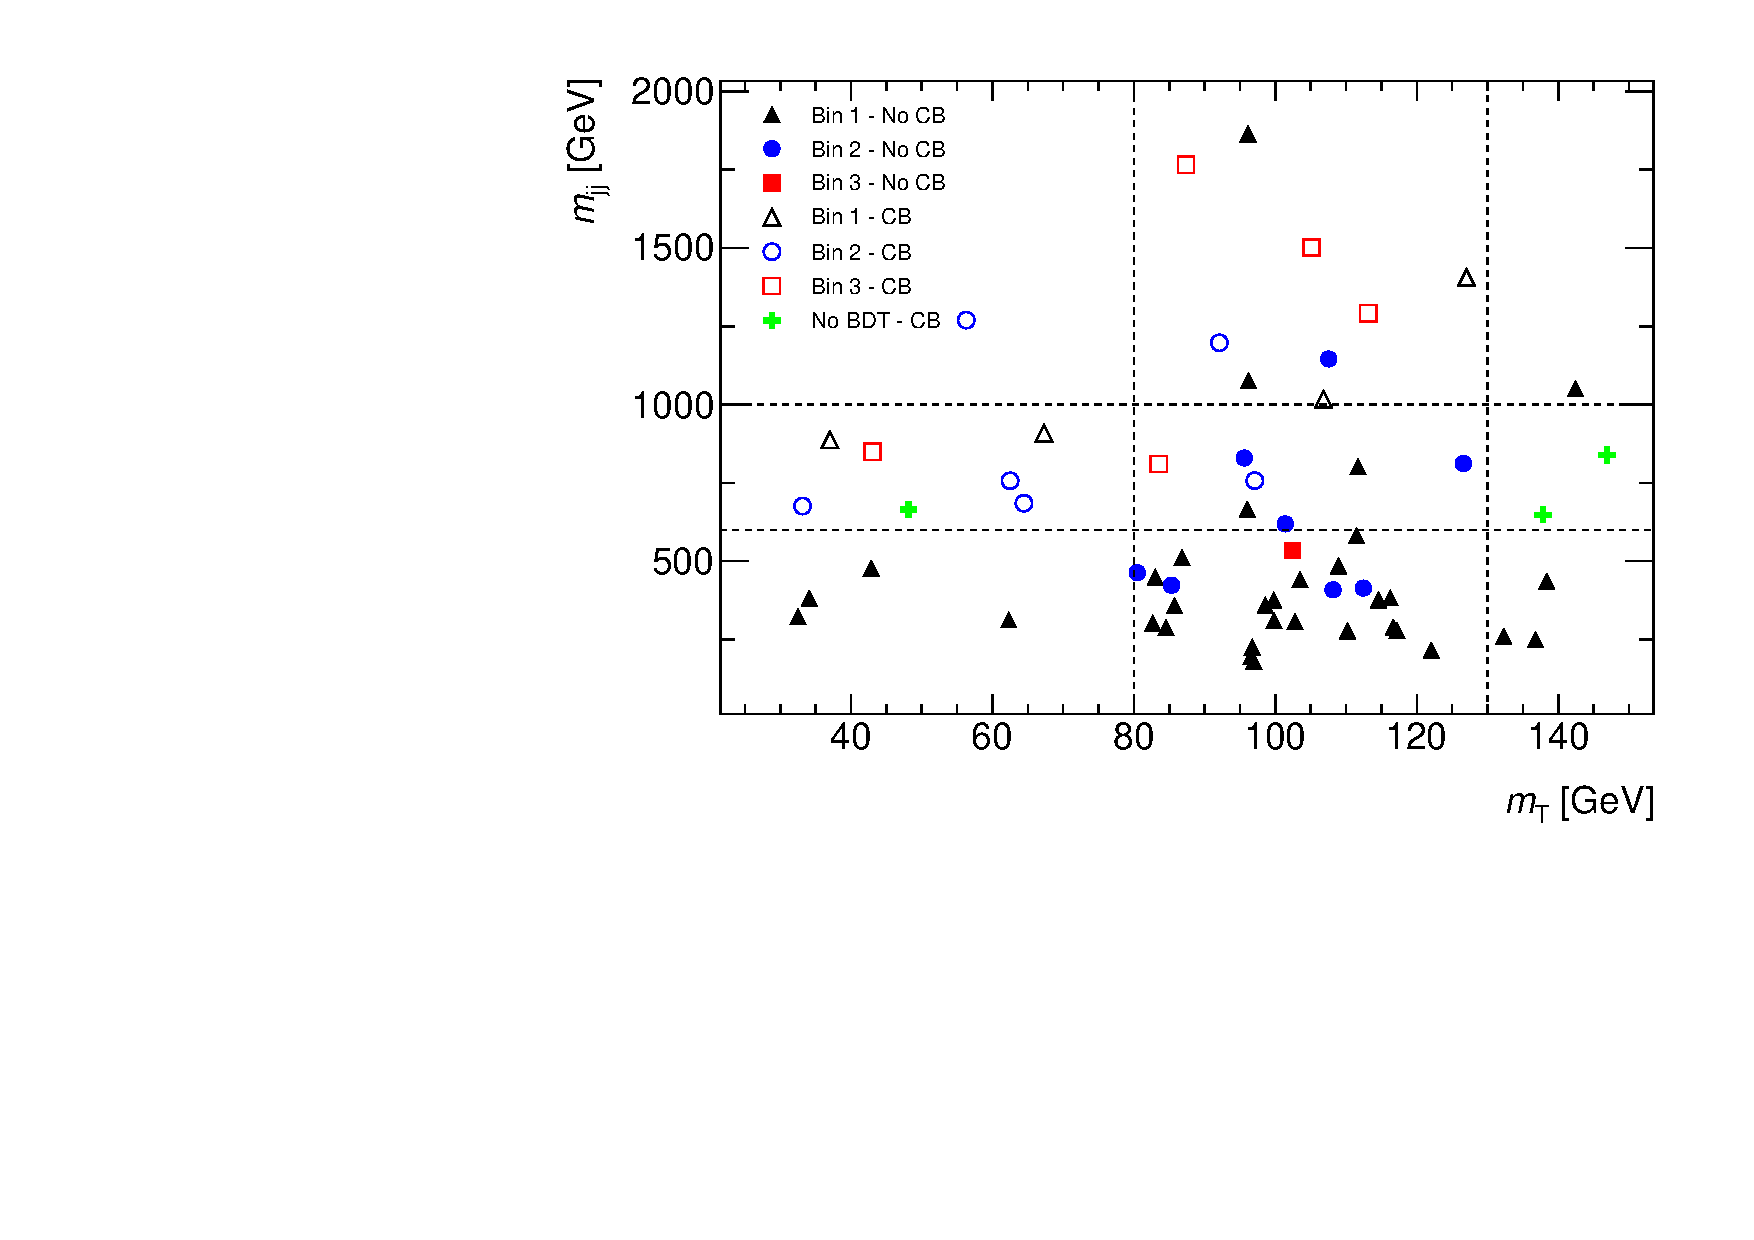
\includegraphics[width=0.8\textwidth]{fig/analysis/data_scatter_mjj_mt.pdf}
\caption{Scatter plot of the \mjj and \mT values for data events falling in
the BDT or cut-based signal regions (\emme channel only). The dashed
lines indicate the binning for the cut-based analysis ($\mjj < 600
\gev$ events fail the selection). Events which fall into BDT bin 1 are
shown in {\bf black}, bin 2 in {\bf\color{blue}blue}, bin 3 in
{\bf\color{red}red}. Solid markers indicate that an event has passed
the BDT selection and not the cut-based selection, and hollow markers
indicate that both have been passed. Finally, events that pass the
cut-based selection and not the BDT are shown in {\bf\color{green}green}.}
\label{chap:analysis:fig:scatterplot_mjj_mt}
\end{figure}

